\documentclass[12pt]{article}

\usepackage{sbc-template}
\usepackage{graphicx,url}
\usepackage[utf8]{inputenc}
\usepackage[T1]{fontenc}
\usepackage[brazil]{babel}
\usepackage{booktabs}
\usepackage{array}
\usepackage{float}

\sloppy

\title{Steam Games Market Insights: Predição e Explicação de Sucesso Comercial de Jogos na Steam}

\author{Davi Silva de Melo Lins\inst{1}, Iury Kauann David Nogueira\inst{1},\\
Isabelle de Lima Xavier\inst{1}, João Raphael Leão Guimarães Oliveira\inst{1},\\
Marcelo Palmeira Falcão\inst{1}}

\address{Curso de Ciência de Dados -- Universidade Federal de Alagoas (UFAL)\\
  Maceió -- AL -- Brasil\\
  \email{\{dsml,ikdn,ilx,jrlgo,mpf\}@ic.ufal.br}
}

\begin{document}

\maketitle

\begin{abstract}
This work analyzes the Steam Games Dataset to support indie developers and publishers in product, pricing and positioning decisions. Commercial success is modeled as a binary proxy, not as real revenue, based on a composite score of estimated owners, reviews, peak concurrent users, recommendations and average playtime. The project compares classical and ensemble classifiers, evaluates them with stratified validation, and extracts actionable insights from descriptive analysis, statistical tests and model interpretation. The best model was the HistGradientBoostingClassifier, with F1-score of 0.7395 and ROC-AUC of 0.9155 on the test set.
\end{abstract}

\begin{resumo}
Este trabalho analisa a base Steam Games Dataset para apoiar desenvolvedores indie e publishers em decisões de produto, preço e posicionamento. O sucesso comercial é modelado como uma proxy binária, não como receita real, baseada em um score composto por donos estimados, avaliações, pico de usuários simultâneos, recomendações e tempo médio de jogo. O projeto compara classificadores clássicos e modelos ensemble, avalia os resultados com validação estratificada e extrai insights acionáveis a partir de análise descritiva, testes estatísticos e interpretabilidade. O melhor modelo foi o HistGradientBoostingClassifier, com F1-score de 0,7395 e ROC-AUC de 0,9155 no conjunto de teste.
\end{resumo}

\section{Introdução e Aplicação}

O mercado de jogos na Steam é competitivo e apresenta forte assimetria de visibilidade. Muitos jogos recebem pouca tração, enquanto uma parcela menor concentra reviews, jogadores, recomendações e engajamento. Para desenvolvedores indie e publishers, esse cenário torna difícil decidir quais características priorizar antes de investir tempo de produção, orçamento de marketing e esforço de comunicação. O problema de negócio deste projeto é apoiar essas decisões com evidências obtidas a partir de jogos já publicados na plataforma.

O público-alvo do trabalho é formado por desenvolvedores independentes, pequenos estúdios e publishers que precisam tomar decisões sobre produto, preço, posicionamento, funcionalidades e estratégia de lançamento. A pergunta de pesquisa é: quais características dos jogos publicados na Steam estão associadas a uma maior probabilidade de sucesso comercial estimado, e como essas evidências podem apoiar decisões de desenvolvimento, posicionamento e publicação? O objetivo é construir um pipeline reprodutível para predizer e explicar a variável \texttt{success\_commercial}, transformando resultados estatísticos e modelos preditivos em recomendações práticas.

A tomada de decisão apoiada não é a aprovação automática de um jogo, mas a priorização de hipóteses de produto e mercado. Por exemplo, os resultados podem ajudar a discutir se vale investir em recursos sociais, como multiplayer, se uma estratégia gratuita é adequada ao gênero, se sistemas de achievements devem ser planejados desde cedo e quais sinais de posicionamento parecem mais relevantes. Todas as interpretações são tratadas como associações observadas no conjunto analisado, não como relações causais.

As hipóteses iniciais do projeto foram: H1, jogos com recursos multiplayer apresentam maior taxa de sucesso comercial estimado; H2, jogos gratuitos e pagos apresentam comportamentos diferentes de sucesso; H3, jogos com achievements apresentam maior taxa de sucesso estimado; H4, tags, gêneros, categorias e recursos da Steam estão associados a diferentes probabilidades de sucesso estimado. Essas hipóteses orientaram a análise exploratória, os testes estatísticos, a engenharia de atributos e a interpretação dos modelos.

\section{Base de Dados}

A base utilizada é o \textit{Steam Games Dataset}, disponível no Kaggle\footnote{\url{https://www.kaggle.com/datasets/fronkongames/steam-games-dataset?resource=download}}. O pipeline usa \texttt{dataset/games.csv} como fonte principal e mantém \texttt{dataset/games.json} apenas como arquivo auxiliar. A pasta \texttt{dataset/} não é versionada no repositório por conter arquivos grandes; para reproduzir o projeto, o usuário deve baixar a base no Kaggle e posicionar os arquivos localmente.

A execução final processou 122.611 registros e 49 colunas após a engenharia de atributos. A taxa positiva da variável-alvo ficou em aproximadamente 30,0\%, coerente com o corte operacional adotado. A base combina variáveis numéricas, categóricas, listas textuais e datas, incluindo preço, data de lançamento, plataformas, owners estimados, reviews, pico de usuários simultâneos, achievements, Metacritic, categorias, gêneros e tags. Durante a leitura, o cabeçalho \texttt{DiscountDLC count} é tratado como duas colunas, \texttt{Discount} e \texttt{DLC count}, sem editar o CSV bruto.

A base é pública e contém registros agregados por jogo/produto. Não há indicação, nos arquivos usados pelo projeto, de dados pessoais sensíveis sobre indivíduos. A licença e os termos de uso devem ser conferidos na página do dataset no Kaggle, sem assumir uma licença específica que não esteja documentada no repositório. Essa observação é importante para a entrega porque o dataset bruto não entra no pacote final: a reprodução depende do download externo e do respeito aos termos da fonte.

\begin{table}[ht]
\centering
\caption{Mini dicionário de dados das principais variáveis.}
\label{tab:dicionario}
\scriptsize
\begin{tabular}{p{0.17\textwidth}p{0.20\textwidth}p{0.13\textwidth}p{0.16\textwidth}p{0.24\textwidth}}
\toprule
Variável & Papel & Tipo & Uso & Observação \\
\midrule
\texttt{Name} & Identificação do jogo & Texto & Descritivo & Não entra no treino \\
\texttt{Price} & Preço do jogo & Numérica & Feature & Origina \texttt{price}, \texttt{log\_price} e \texttt{free\_to\_play} \\
\texttt{Release date} & Data de lançamento & Data/texto & Feature derivada & Origina \texttt{release\_year} e \texttt{game\_age\_years} \\
\texttt{Genres} & Gêneros declarados & Lista/texto & Feature derivada & Usada em contagens e flags de taxonomia \\
\texttt{Tags} & Tags da Steam & Lista/texto & Feature derivada & Usada em \texttt{tag\_count} e flags de gênero/tema \\
\texttt{Categories} & Recursos da Steam & Lista/texto & Feature derivada & Usada para multiplayer, achievements, cloud e cards \\
\texttt{Positive} & Reviews positivas & Numérica & Proxy/EDA & Removida das features por vazamento \\
\texttt{Negative} & Reviews negativas & Numérica & Proxy/EDA & Removida das features por vazamento \\
\texttt{Recommendations} & Recomendações & Numérica & Proxy & Removida das features por vazamento \\
\texttt{Peak CCU} & Pico de usuários simultâneos & Numérica & Proxy & Removida das features por vazamento \\
\texttt{Average playtime forever} & Tempo médio de jogo & Numérica & Proxy & Removida das features por vazamento \\
\texttt{Estimated owners} & Faixa estimada de donos & Faixa & Proxy & Convertida em midpoint e removida das features \\
\texttt{success\_commercial} & Sucesso estimado & Binária & Alvo & Proxy top 30\%, não receita real \\
\bottomrule
\end{tabular}
\end{table}

\section{Definição da Variável-Alvo}

A variável-alvo \texttt{success\_commercial} é uma proxy binária de sucesso comercial, não uma medida de receita real. Ela foi criada a partir do score composto \texttt{commercial\_success\_score}, calculado com cinco componentes: ponto médio de \texttt{Estimated owners} (\texttt{owners\_midpoint}), \texttt{total\_reviews}, \texttt{peak\_ccu}, \texttt{recommendations} e \texttt{average\_playtime\_forever}. Esses componentes representam sinais complementares de alcance, atenção do público e engajamento.

Cada componente passa por transformação \texttt{log1p}, para reduzir o peso de outliers extremos, e depois é convertido em ranking percentual dentro da base. O score final é a média simples desses rankings. Um jogo recebe \texttt{success\_commercial = 1} quando seu score composto está no top 30\% da base, isto é, acima do quantil 70. Na execução final, o corte foi 0,524124 e a proporção positiva resultante foi aproximadamente 30,0\%.

A definição composta foi escolhida porque \texttt{Estimated owners} sozinho possui faixas largas e muitos empates, especialmente na faixa inferior. Usar apenas owners estimados também poderia favorecer jogos com grande alcance, mas pouco engajamento ou baixa avaliação pública. A combinação de owners estimados, reviews, pico de usuários, recomendações e tempo médio de jogo permite capturar dimensões diferentes do desempenho. Ainda assim, a definição tem limitações: owners é uma estimativa em faixa, reviews e recomendações podem favorecer jogos antigos ou muito expostos, e engajamento não substitui faturamento.

A escolha do top 30\% tem caráter operacional. Ela cria uma classe positiva relevante para o problema de negócio, mas ainda com tamanho suficiente para treinamento e avaliação dos modelos. Um corte muito restritivo, como top 10\%, poderia aproximar a classe positiva de grandes sucessos, porém reduziria a quantidade de exemplos e tornaria a classificação mais instável. Um corte muito amplo, como top 50\%, tornaria o alvo menos seletivo e menos conectado à ideia de destaque comercial.

\section{Pré-processamento e Engenharia de Atributos}

A preparação dos dados incluiu conversão numérica de colunas como preço, reviews, Metacritic, achievements, recomendações e tempo de jogo; parsing de datas de lançamento; parsing das faixas de owners; e parsing de listas de categorias, gêneros, tags, idiomas e áudio. A partir dessas listas foram criadas contagens e indicadores binários, como \texttt{has\_multiplayer}, \texttt{has\_singleplayer}, \texttt{is\_indie}, \texttt{is\_action}, \texttt{has\_steam\_cloud}, \texttt{has\_trading\_cards} e \texttt{has\_family\_sharing}.

O tratamento de nulos foi realizado principalmente por preenchimentos específicos na engenharia de atributos e por imputação mediana dentro dos pipelines de modelagem. Valores negativos em variáveis como preço e contagens foram limitados inferiormente a zero. Outliers foram mitigados por transformações logarítmicas, pelo uso de ranking percentual no score-alvo e por visualizações com corte no percentil 99 para preço; não houve remoção agressiva de observações extremas. Não foi documentada uma etapa específica de deduplicação, o que permanece como limitação para usos produtivos futuros.

Para evitar vazamento de dados, foram removidas da matriz de modelagem as colunas usadas diretamente na criação da variável-alvo e suas derivadas: \texttt{Estimated owners}, \texttt{owners\_lower}, \texttt{owners\_upper}, \texttt{owners\_midpoint}, \texttt{Peak CCU}, \texttt{peak\_ccu}, \texttt{Positive}, \texttt{Negative}, \texttt{positive\_reviews}, \texttt{negative\_reviews}, \texttt{total\_reviews}, \texttt{review\_score\_weighted}, \texttt{positive\_ratio}, \texttt{Recommendations}, \texttt{recommendations}, \texttt{Average playtime forever}, \texttt{average\_playtime\_forever}, o score composto e o próprio alvo. A remoção de \texttt{positive\_ratio} é especialmente importante por ser derivada diretamente de \texttt{Positive} e \texttt{Negative}.

As features finais incluem informações de preço, ano/idade do jogo, plataformas, contagens de taxonomia, idiomas, achievements, Metacritic, recursos da Steam e indicadores de gênero/tema. A escolha dessas features preserva a compatibilidade entre modelos lineares, árvores e métodos ensemble, permitindo comparação justa dentro de pipelines de pré-processamento. Para uso pré-lançamento, uma versão futura deveria restringir ainda mais as features a variáveis conhecidas antes da publicação, pois alguns campos atuais refletem desempenho posterior ao lançamento.

\section{Análise Exploratória e Inferência}

A Figura~\ref{fig:target} mostra a distribuição da variável-alvo, coerente com o corte operacional de top 30\%. As comparações entre grupos indicam padrões relevantes para decisão de produto e posicionamento. Jogos com multiplayer apresentaram taxa de sucesso de 44,9\%, contra 26,7\% nos demais jogos. Jogos gratuitos apresentaram taxa de sucesso de 17,6\%, enquanto jogos pagos apresentaram 33,4\%. Jogos com achievements apresentaram 40,1\%, contra 19,3\% nos jogos sem achievements.

\begin{figure}[ht]
\centering
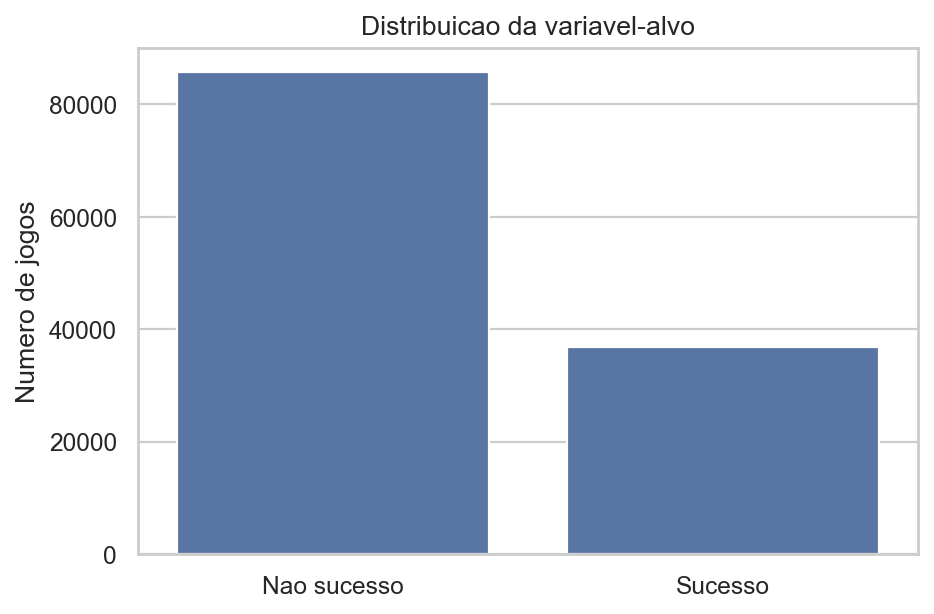
\includegraphics[width=.58\textwidth]{images/target_distribution.png}
\caption{Distribuição da variável-alvo \texttt{success\_commercial}.}
\label{fig:target}
\end{figure}

\begin{figure}[ht]
\centering
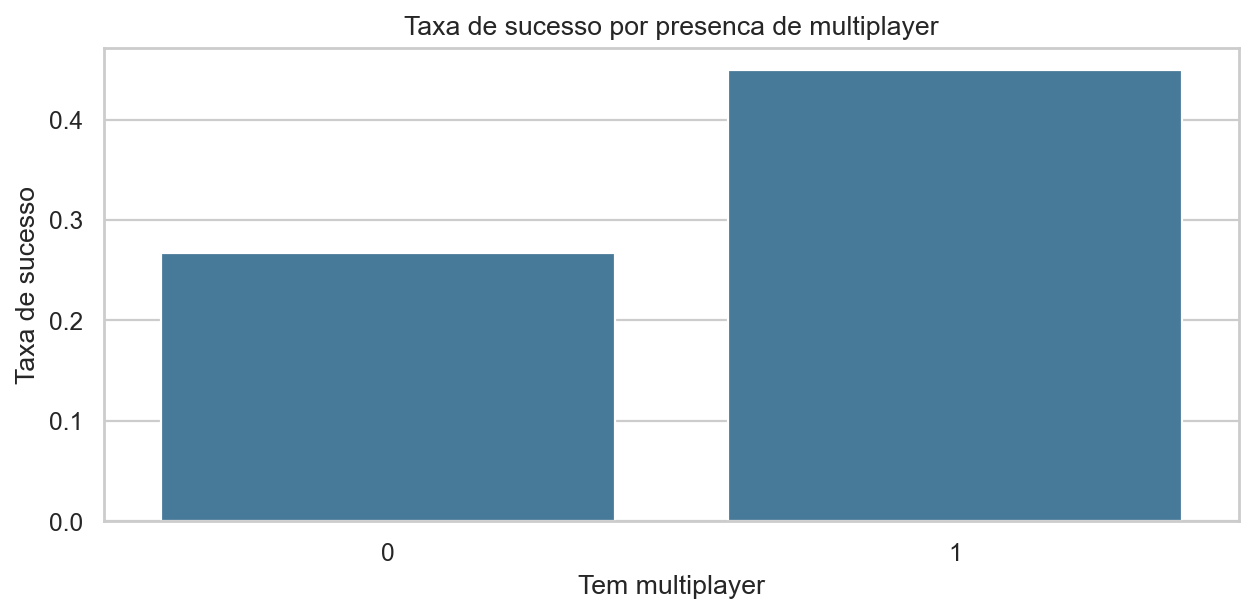
\includegraphics[width=.48\textwidth]{images/success_rate_multiplayer.png}\hfill
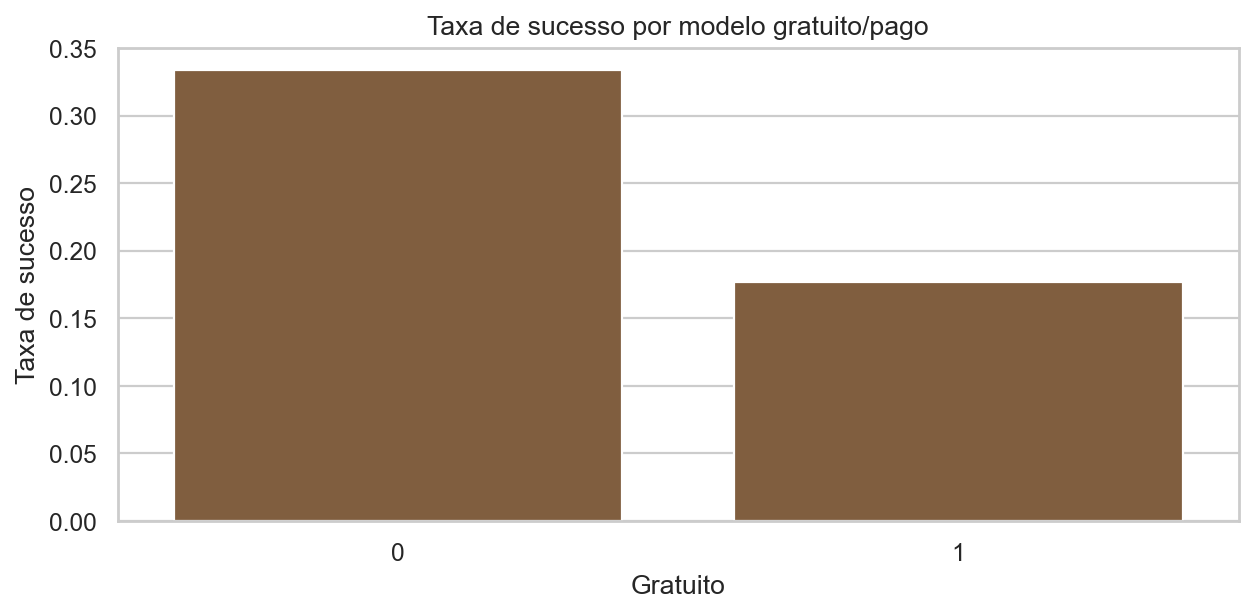
\includegraphics[width=.48\textwidth]{images/success_rate_free_to_play.png}
\caption{Taxas de sucesso por presença de multiplayer e por modelo gratuito/pago.}
\label{fig:groups}
\end{figure}

A Tabela~\ref{tab:grupos} resume comparações descritivas centrais. As diferenças não devem ser lidas isoladamente como recomendação universal. Por exemplo, a menor taxa observada em jogos gratuitos não significa que todo jogo pago terá melhor desempenho; ela sugere que o modelo de preço precisa ser analisado junto ao gênero, à monetização e ao público-alvo. Da mesma forma, a associação observada para multiplayer não implica que todo jogo deva incluir modo online.

\begin{table}[ht]
\centering
\caption{Comparações descritivas entre grupos selecionados.}
\label{tab:grupos}
\scriptsize
\begin{tabular}{lrrrr}
\toprule
Grupo & Valor & Jogos & Taxa de sucesso & Mediana de reviews \\
\midrule
Gratuito & Não & 96.405 & 33,4\% & 10 \\
Gratuito & Sim & 26.206 & 17,6\% & 0 \\
Multiplayer & Não & 100.654 & 26,7\% & 5 \\
Multiplayer & Sim & 21.957 & 44,9\% & 22 \\
Achievements & Não & 59.572 & 19,3\% & 2 \\
Achievements & Sim & 63.039 & 40,1\% & 17 \\
\bottomrule
\end{tabular}
\end{table}

As hipóteses foram avaliadas com EDA, testes estatísticos e modelagem, sempre com linguagem associativa. A Tabela~\ref{tab:testes} resume os testes principais. O p-valor foi reportado como \(p < 10^{-300}\) quando o valor numérico exportado ficou igual a zero por limite de precisão. Esses resultados indicam associação estatística, mas não permitem concluir causalidade.

\begin{table}[ht]
\centering
\caption{Testes estatísticos principais.}
\label{tab:testes}
\scriptsize
\begin{tabular}{p{0.18\textwidth}p{0.45\textwidth}p{0.15\textwidth}p{0.12\textwidth}}
\toprule
Teste & Comparação & Estatística & p-valor \\
\midrule
Mann-Whitney U & Score comercial: multiplayer vs. não multiplayer & 1.377.274.066 & $<10^{-300}$ \\
Mann-Whitney U & Score comercial: gratuitos vs. pagos & 615.574.825 & $<10^{-300}$ \\
Mann-Whitney U & Score comercial: indie vs. não indie & 1.977.259.432 & $<10^{-300}$ \\
Qui-quadrado & Sucesso comercial vs. multiplayer & 2.830,52 & $<10^{-300}$ \\
Qui-quadrado & Sucesso comercial vs. gratuito & 2.420,71 & $<10^{-300}$ \\
\bottomrule
\end{tabular}
\end{table}

\section{Modelagem e Avaliação}

A tarefa foi formulada como classificação binária. Foram avaliados cinco modelos principais: Regressão Logística como baseline linear, Árvore de Decisão como baseline interpretável, Random Forest, Extra Trees e HistGradientBoostingClassifier. XGBoost e LightGBM são opcionais no pipeline, mas não foram considerados como dependências obrigatórias. Essa seleção cobre modelos simples, modelos interpretáveis e ensembles mais robustos para relações não lineares.

A avaliação usou split treino/teste estratificado, com 20\% da base reservado para teste, e validação cruzada estratificada com 3 folds no conjunto de treino. A reprodutibilidade foi controlada com \texttt{random\_state=42}. Para lidar com a classe positiva de aproximadamente 30\%, os modelos que suportam pesos usaram configurações balanceadas, como \texttt{class\_weight=balanced} ou \texttt{balanced\_subsample}. As métricas reportadas foram accuracy, precision, recall, F1-score, ROC-AUC e matriz de confusão.

A escolha do F1-score e da ROC-AUC como critérios principais decorre do problema de negócio. Accuracy pode parecer alta mesmo quando o modelo erra muitos casos positivos em bases desbalanceadas. Precision mede a confiabilidade das previsões positivas, enquanto recall mede a capacidade de recuperar jogos que pertencem à classe de sucesso estimado. O F1-score resume o equilíbrio entre precision e recall, e a ROC-AUC avalia a capacidade discriminativa global do modelo.

\begin{table}[ht]
\centering
\caption{Métricas no conjunto de teste.}
\label{tab:metricas}
\scriptsize
\begin{tabular}{lccccc}
\toprule
Modelo & Accuracy & Precision & Recall & F1 & ROC-AUC \\
\midrule
HistGradientBoosting & 0,8285 & 0,6793 & 0,8115 & 0,7395 & 0,9155 \\
Random Forest & 0,8307 & 0,6945 & 0,7780 & 0,7339 & 0,9117 \\
Extra Trees & 0,8143 & 0,6613 & 0,7809 & 0,7162 & 0,9008 \\
Regressão Logística & 0,8008 & 0,6381 & 0,7763 & 0,7004 & 0,8862 \\
Árvore de Decisão & 0,7949 & 0,6257 & 0,7877 & 0,6974 & 0,8880 \\
\bottomrule
\end{tabular}
\end{table}

A Figura~\ref{fig:metricas} complementa a Tabela~\ref{tab:metricas} com uma comparação visual das métricas dos modelos avaliados. A Tabela~\ref{tab:cv} mostra que o desempenho observado no teste também é compatível com a validação cruzada no conjunto de treino, reduzindo o risco de escolher o modelo apenas por uma divisão específica dos dados.

\begin{figure}[ht]
\centering
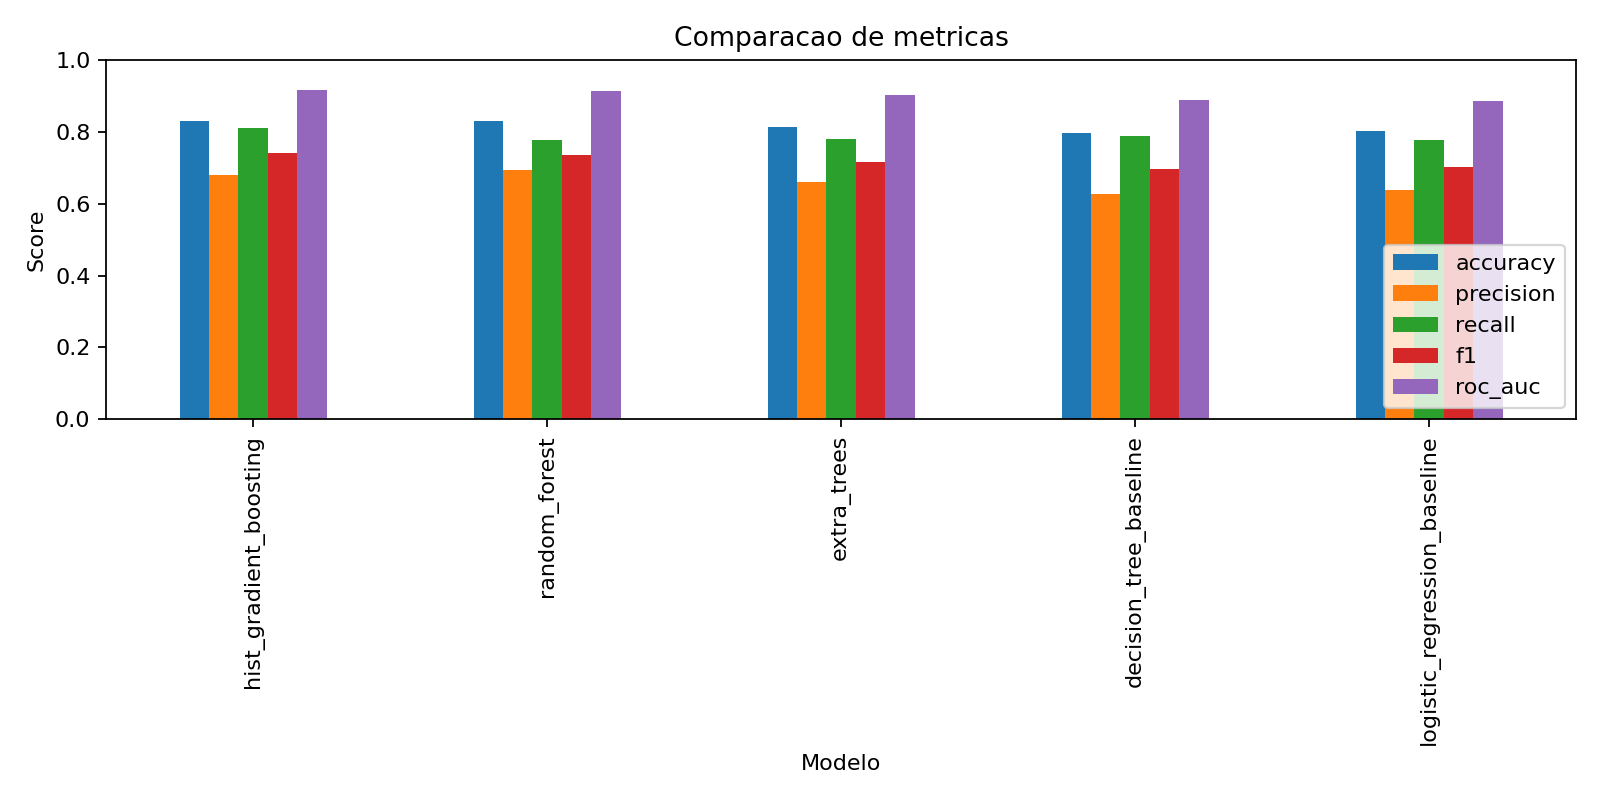
\includegraphics[width=.72\textwidth]{images/metrics_bar_chart.png}
\caption{Comparação visual das métricas dos modelos avaliados.}
\label{fig:metricas}
\end{figure}

\begin{table}[ht]
\centering
\caption{Validação cruzada estratificada com 3 folds no conjunto de treino.}
\label{tab:cv}
\scriptsize
\begin{tabular}{lccc}
\toprule
Modelo & F1 médio & ROC-AUC médio & Accuracy média \\
\midrule
Regressão Logística & 0,7006 & 0,8867 & 0,8011 \\
Árvore de Decisão & 0,6964 & 0,8860 & 0,7965 \\
Random Forest & 0,7356 & 0,9098 & 0,8318 \\
Extra Trees & 0,7205 & 0,9017 & 0,8171 \\
HistGradientBoosting & 0,7389 & 0,9144 & 0,8280 \\
\bottomrule
\end{tabular}
\end{table}

\begin{figure}[ht]
\centering
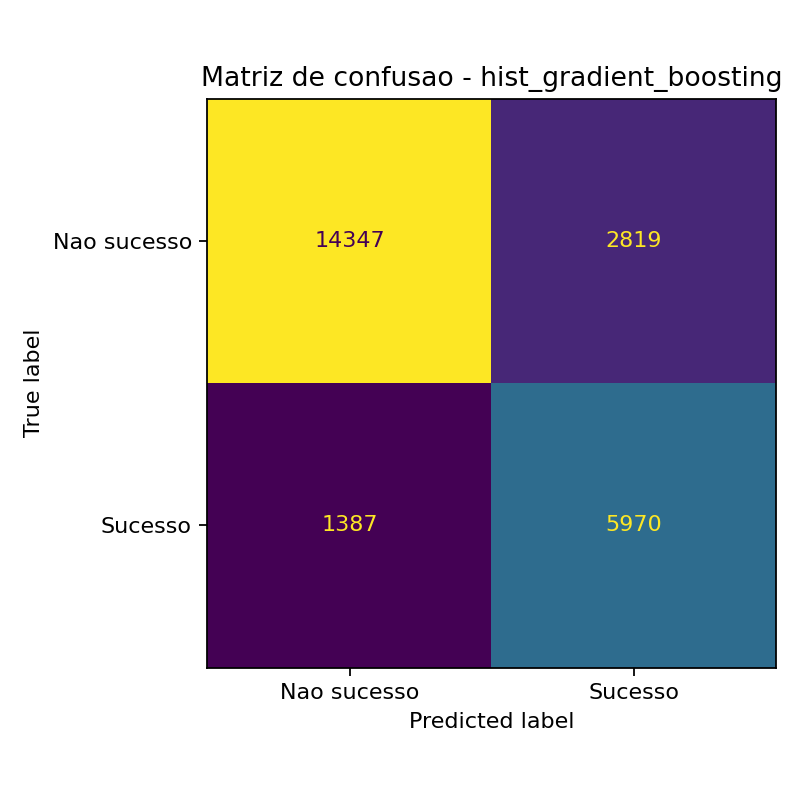
\includegraphics[width=.52\textwidth]{images/best_model_confusion_matrix.png}
\caption{Matriz de confusão do melhor modelo no conjunto de teste.}
\label{fig:confusao}
\end{figure}

\section{Resultados e Discussão}

O melhor modelo atual foi o HistGradientBoostingClassifier, identificado no pipeline como \texttt{hist\_gradient\_boosting}. Ele obteve F1-score de 0,7395 e ROC-AUC de 0,9155, superando os demais modelos nesses critérios. A Random Forest apresentou accuracy e precision ligeiramente maiores, 0,8307 e 0,6945, respectivamente, mas o HistGradientBoosting apresentou melhor equilíbrio entre recuperação da classe positiva e capacidade discriminativa global.

Falsos positivos representam jogos previstos como sucesso que não pertencem à classe de sucesso estimado. No contexto de negócio, isso pode gerar expectativa excessiva e levar a investimentos de produto ou marketing que exigem validação complementar. Falsos negativos representam jogos previstos como não sucesso que pertencem à classe de sucesso estimado; o risco é ignorar oportunidades promissoras. Como o objetivo é apoiar decisão estratégica, esses erros devem ser tratados como alertas para análise humana, considerando gênero, público-alvo e estratégia de lançamento.

A Figura~\ref{fig:confusao} apresenta a matriz de confusão do melhor modelo no conjunto de teste. O modelo classificou corretamente 14.347 jogos da classe negativa e 5.970 jogos da classe positiva. Também houve 2.819 falsos positivos e 1.387 falsos negativos. Essa configuração favorece bom recall para a classe positiva, característica útil quando o objetivo é identificar oportunidades para análise posterior, e não automatizar decisões finais de investimento.

A interpretabilidade do melhor modelo foi analisada por importância de features. As variáveis mais relevantes foram \texttt{tag\_count}, \texttt{game\_age\_years}, \texttt{has\_trading\_cards}, \texttt{price} e \texttt{discount}. Em linguagem de negócio, isso sugere que posicionamento por tags, maturidade histórica do jogo, recursos da Steam e preço estão associados a padrões de desempenho na base. Esses fatores não devem ser lidos como causas diretas.

\begin{figure}[ht]
\centering
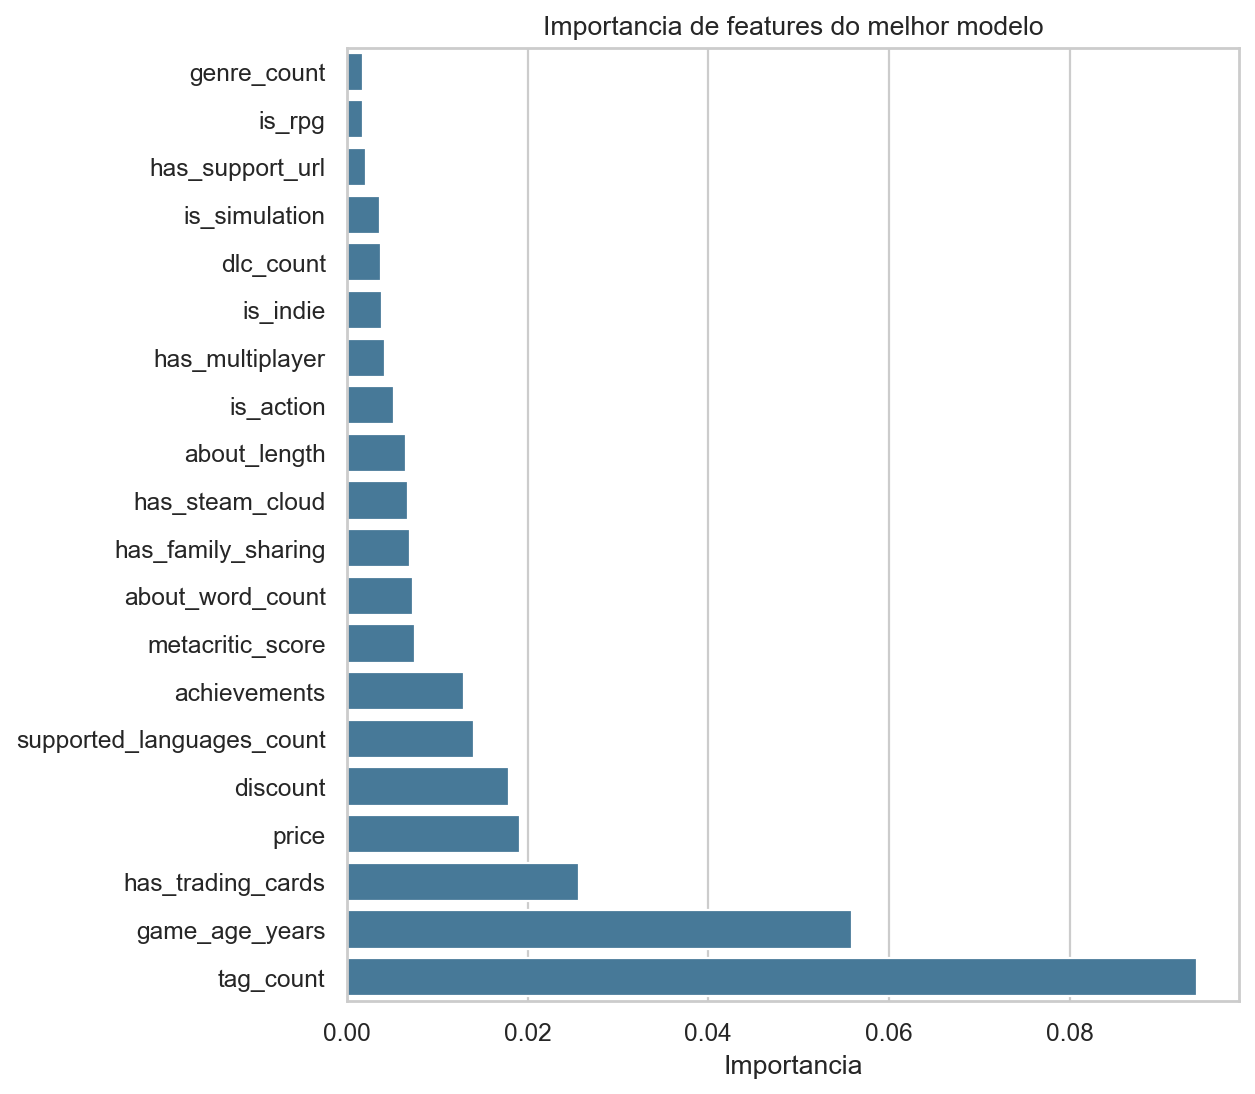
\includegraphics[width=.75\textwidth]{images/feature_importance.png}
\caption{Importância de features do melhor modelo.}
\label{fig:importance}
\end{figure}

\begin{table}[ht]
\centering
\caption{Principais features por importância no melhor modelo.}
\label{tab:importance}
\scriptsize
\begin{tabular}{lr}
\toprule
Feature & Importância \\
\midrule
\texttt{tag\_count} & 0,0941 \\
\texttt{game\_age\_years} & 0,0559 \\
\texttt{has\_trading\_cards} & 0,0257 \\
\texttt{price} & 0,0191 \\
\texttt{discount} & 0,0179 \\
\texttt{supported\_languages\_count} & 0,0141 \\
\texttt{achievements} & 0,0129 \\
\texttt{metacritic\_score} & 0,0075 \\
\bottomrule
\end{tabular}
\end{table}

A presença de \texttt{tag\_count} como feature mais importante sugere que a taxonomia do jogo na Steam é um sinal relevante para o modelo. Isso pode refletir melhor descrição do produto, maior granularidade de posicionamento ou maior complexidade de gêneros e temas. A variável \texttt{game\_age\_years} deve ser interpretada com cuidado, pois jogos antigos tiveram mais tempo para acumular reviews, owners e reconhecimento. Já \texttt{has\_trading\_cards}, \texttt{achievements} e \texttt{has\_steam\_cloud} indicam recursos de plataforma que podem estar associados a acabamento percebido, engajamento ou maturidade de publicação.

As principais limitações são a ausência de receita real, o uso de uma proxy operacional, a presença de variáveis pós-lançamento, possível viés de popularidade e a ausência de uma etapa documentada de deduplicação. Para uso pré-lançamento, seria necessário treinar uma versão restrita a features disponíveis antes da publicação do jogo. Também seria útil calibrar probabilidades, testar segmentações por gênero e avaliar estabilidade temporal, pois o mercado de jogos muda rapidamente.

\section{Insights Acionáveis}

O primeiro insight é que jogos com multiplayer apresentaram maior taxa de sucesso estimado no conjunto analisado: 44,9\% contra 26,7\% nos demais. Isso sugere que recursos sociais podem estar associados a retenção, descoberta e recorrência. A recomendação é avaliar modos cooperativos, competitivos ou eventos online quando fizerem sentido para o gênero. Após 6 meses do lançamento, a ação pode ser avaliada por pico de usuários simultâneos, reviews e retenção; a meta operacional sugerida é superar em pelo menos 10\% a taxa média de sucesso do segmento.

O segundo insight é que jogos gratuitos apresentaram taxa de sucesso menor que jogos pagos na base analisada: 17,6\% contra 33,4\%. Isso sugere que preço zero não deve ser adotado automaticamente como estratégia de sucesso. A recomendação é testar preços de entrada baixos, demos ou períodos promocionais, considerando gênero e modelo de monetização. Após 3 meses, a avaliação deve observar conversão, reviews, donos estimados e receita por usuário, quando disponível.

O terceiro insight é que jogos com achievements apresentaram taxa de sucesso de 40,1\%, contra 19,3\% nos jogos sem achievements. Isso sugere associação entre sistemas de progresso, acabamento percebido e engajamento. A recomendação é planejar achievements conectados a marcos reais de gameplay, evitando conquistas artificiais. Após 3 meses, a ação pode ser avaliada por tempo médio de jogo e proporção de jogadores que desbloqueiam conquistas intermediárias.

Esses insights devem ser usados como hipóteses priorizadas, não como regras universais. Para um desenvolvedor indie, o valor prático está em reduzir incerteza: antes de investir em uma funcionalidade, o time pode perguntar se ela faz sentido para o gênero, se há evidência de associação positiva no histórico da Steam e como o impacto será medido depois do lançamento. Para um publisher, os resultados ajudam a estruturar conversas sobre posicionamento, calendário de lançamento, estratégia de preço e riscos de comunicação.

\section{Recurso Extra}

Como recurso extra, o projeto inclui uma aplicação local em Streamlit. O app permite carregar \texttt{dataset/games.csv} ou enviar um CSV compatível, selecionar modelos, treinar classificadores, visualizar métricas e gerar gráficos com Matplotlib. O app utiliza a mesma definição de \texttt{success\_commercial} e preserva a remoção de colunas com risco de vazamento.

A aplicação também possui geração opcional de relatório automatizado com Gemini. A chave é configurada localmente via \texttt{.env} a partir de \texttt{.env.example}; o app funciona sem chave, desativando apenas a geração do relatório. Apenas informações agregadas, como métricas, melhor modelo, features principais e resumo do alvo, são enviadas ao Gemini. Esse relatório é um artefato auxiliar de comunicação e não foi usado como fonte principal da análise.

Esse recurso extra reforça a reprodutibilidade e a comunicação do projeto. Em uma situação de apresentação para banca ou para um publisher, o app permite demonstrar rapidamente como diferentes modelos se comparam e como as métricas são traduzidas em gráficos. Ainda assim, o app não substitui o relatório técnico, pois as decisões metodológicas, limitações e interpretações precisam permanecer documentadas no texto principal.


\subsection{Uso dos resultados na prática}

Os resultados do projeto devem ser usados como apoio à triagem, à priorização e à reflexão estratégica, não como decisão automática. Como \texttt{success\_commercial} é uma proxy de sucesso comercial e não receita real, as previsões ajudam a organizar hipóteses sobre produto, preço, posicionamento e recursos, mas não garantem desempenho futuro. Antes de transformar uma recomendação em investimento, desenvolvedores e publishers devem considerar gênero, público-alvo, orçamento, calendário de lançamento e estratégia de marketing.

Na prática, o modelo pode funcionar como um radar inicial. Jogos ou conceitos com maior potencial estimado podem ser priorizados para análise humana mais detalhada, enquanto sinais de risco podem orientar testes de comunicação, preço ou escopo. O acompanhamento deve ocorrer após o lançamento ou após mudanças de posicionamento, usando métricas observáveis como reviews, retenção, conversão da página e engajamento. As associações observadas no conjunto analisado não devem ser interpretadas como causalidade.

\begin{table}[ht]
\centering
\caption{Exemplos de uso prático dos resultados para tomada de decisão.}
\label{tab:uso-pratico}
\scriptsize
\begin{tabular}{p{0.20\textwidth}p{0.25\textwidth}p{0.27\textwidth}p{0.18\textwidth}}
\toprule
Decisão apoiada & Evidência utilizada & Ação sugerida & Métrica de acompanhamento \\
\midrule
Priorização de recursos do produto & Maior taxa de sucesso em jogos com multiplayer/achievements, quando aplicável & Avaliar se esses recursos fazem sentido para o gênero e escopo do jogo & Reviews positivas, retenção e engajamento \\
Estratégia de preço e posicionamento & Diferença observada entre jogos pagos e gratuitos & Testar cenários de preço, desconto e percepção de valor & Conversão, reviews, owners estimados e receita observada, quando disponível \\
Seleção de nicho e comunicação & Tags, gêneros e categorias relevantes no modelo & Ajustar página da Steam, tags e mensagens de marketing & Wishlist, conversão da página, reviews e engajamento \\
Triagem de portfólio & Probabilidade estimada pelo modelo e importância das features & Priorizar análise humana dos jogos ou projetos com maior potencial estimado & Desempenho real após 3 ou 6 meses \\
\bottomrule
\end{tabular}
\end{table}

\section{Conclusão}

O projeto construiu um pipeline reprodutível para predizer e explicar uma proxy de sucesso comercial de jogos na Steam. A definição de \texttt{success\_commercial} combina sinais complementares de alcance e engajamento, evitando depender somente de owners estimados. O melhor modelo foi o HistGradientBoostingClassifier, com ROC-AUC de 0,9155 e F1-score de 0,7395 no conjunto de teste.

Os achados indicam que multiplayer, estratégia de preço, achievements, taxonomia por tags e recursos da Steam estão associados a diferenças de desempenho na base analisada. A decisão recomendada é usar esses resultados como apoio para priorizar hipóteses de produto e posicionamento, sempre combinando o modelo com análise de gênero, público-alvo e estratégia comercial. Em termos práticos, o projeto não entrega uma fórmula de sucesso, mas um mapa de evidências para reduzir incerteza e orientar experimentos.

As limitações principais envolvem a ausência de receita real, a natureza aproximada da variável-alvo, a presença de variáveis pós-lançamento e a necessidade de validação em cenários específicos. Trabalhos futuros podem incluir uma versão pré-lançamento do modelo, checagem formal de duplicatas, calibração de probabilidades, estimativas de receita com hipóteses explícitas, análise temporal, exploração segmentada por gênero e integração com dashboards interativos.

\begin{thebibliography}{9}

\bibitem{kaggle-steam}
Fronkon Games. \textit{Steam Games Dataset}. Kaggle. Disponível em: \url{https://www.kaggle.com/datasets/fronkongames/steam-games-dataset?resource=download}. Acesso em: 2026.

\bibitem{scikit-learn}
Scikit-learn Developers. \textit{Scikit-learn: Machine Learning in Python}. Disponível em: \url{https://scikit-learn.org/}.

\bibitem{scipy}
SciPy Developers. \textit{SciPy Documentation}. Disponível em: \url{https://docs.scipy.org/doc/scipy/}.

\bibitem{streamlit}
Streamlit. \textit{Streamlit Documentation}. Disponível em: \url{https://docs.streamlit.io/}.

\bibitem{sbc}
Sociedade Brasileira de Computação. \textit{Template para artigos SBC}. Arquivos do template fornecidos na disciplina.

\end{thebibliography}

\end{document}
